\documentclass[../pde_notes.tex]{subfiles}
\begin{document}
\section{Aula 11 - 07 de Abril, 2025}
\subsection{Motivações}
\begin{itemize}
	\item Existência e Unicidade da Solução do Calor;
	\item Equação da Onda.
\end{itemize}
\subsection{Existência e Unicidade da Solução do Calor.}
Na aula passada, aplicamos o método da energia/princípio do máximo à equação do calor
\[
	\left\{\begin{array}{ll}
		\frac{\partial^{}u}{\partial t^{}}(x, t) = \frac{\partial^{2}u}{\partial x^{2}},            & \quad x\in[0, \pi ],\; t>0 \\
		\frac{\partial^{}u}{\partial x^{}}(0, t) = \frac{\partial^{}u}{\partial x^{}}(\pi , t) = 0, & \quad t>0                  \\
		u(x, 0) = u_{0}(x),                                                                         & \quad x\in [0, \pi ]
	\end{array}\right.
\]
para provar a unicidade de sua solução, e a separação de variáveis para a existência. Neste processo, obtivemos a suposta solução
\[
	u(x, t) = \sum\limits_{n=1}^{\infty}b_{n}e^{-n^{2}t}\sin^{}{(nx)},\quad b_{n} = \int_{0}^{\pi }u_{0}(y)\sin^{}{(ny)}.
\]
Sendo assim, devemos conferir se ela é realmente uma solução! Quanto à condição de contorno,
\begin{align*}
	 & u(0, t) = \sum\limits_{n=1}^{\infty}b_{n}e^{-n^{2}t}\sin^{}{(n0)} = 0        \\
	 & u(\pi , t) = \sum\limits_{n=1}^{\infty}b_{n}e^{-n^{2}t}\sin^{}{(n\pi )} = 0.
\end{align*}
Para a condição inicial, olhamos para a extensão ímpar \(2\pi \)-periódica da função \(u_{0}\). Vimos que:
\begin{itemize}
	\item[1)] Se \(u_{0}\) é contínua por partes,
	      \[
		      \int_{0}^{\pi }\biggl\vert u_{0}(x) - \sum\limits_{n=1}^{N}b_{n}\sin^{}{(nx)} \biggr\vert^{2}dx \overbracket[0pt]{\longrightarrow}^{N\to \infty}0;
	      \]
	\item[2)] Se \(u_{0}\) é suave por partes,
	      \[
		      \sum\limits_{n=1}^{\infty}b_{n}\sin^{}{(nx)} = \frac{u_{0}(x^{+}) + u_{0}(x^{-})}{2}.
	      \]
	\item[3)] Se \(u_{0}\) é uma função contínua e também suave por partes, supondo \(u_{0}(0) = u_{0}(\pi ) = 0\), então temos a convergência uniforme
	      \[
		      \lim_{N\to \infty}\biggl(\max_{x\in [0, \pi ]}\biggl\vert \sum\limits_{n=1}^{N}b_{n}\sin^{}{(nx)}-u_{0}(x) \biggr\vert\biggr) = 0.
	      \]
\end{itemize}
\begin{tcolorbox}[
		skin=enhanced,
		title=Lembrete!,
		after title={\hfill Troca de j-ésima derivada com limite},
		fonttitle=\bfseries,
		sharp corners=downhill,
		colframe=black,
		colbacktitle=yellow!75!white,
		colback=yellow!30,
		colbacklower=black,
		coltitle=black,
		%drop fuzzy shadow,
		drop large lifted shadow
	]
	Considere a sequência de funções \((f_{n})_{n\in \mathbb{N}},\; f_{n}:[a, b]\rightarrow \mathbb{R}\) em que cada \(f_{n}\) é \(\mathcal{C}^{k}\). Suponha que todas as derivadas, até a k-ésima, convergem uniformemente para a respectiva derivada de uma mesma função:
	\[
		\forall j\in \{0,\dotsc ,k\},\quad \frac{d^{j}f_{n}}{dx^{j}}\overbracket[0pt]{\longrightarrow}^{n\to \infty}f^{(j)}:[a, b]\rightarrow \mathbb{R}.
	\]
	Logo, \(f = f^{(0)}\) é também de ordem \(\mathcal{C}^{k}\) e
	\[
		\frac{d^{j}f}{dx^{j}} = f^{(j)}.
	\]
	A conclusão é que podemos trocar a ordem de realizar a j-ésima derivada antes ou depois do limite da sequência de funções:
	\[
		\frac{d^{j}}{dx^{j}}(\lim_{n\to \infty}f_{n}) = \lim_{n\to \infty}\biggl(\frac{d^{j}f}{dx^{j}}\biggr).
	\]
	O mesmo resultado vale para funções de várias variáveis, como \(u:[0, \pi ]\times [t_{0}, \infty)\rightarrow \mathbb{R}\), em que \(t_{0}\) é positivo, desde que todas as derivadas parciais até a (k+j)-ésima com respeito à t e à x, convirjam uniformemente.
\end{tcolorbox}

(Lembramos que, conforme fora dito em alguma nota de rodapé, ou num lembrete, dizer que uma função é suave vai à gosto do material sendo usado). Agora, vamos mostrar que
\[
	\sum\limits_{n=1}^{\infty}\frac{\partial^{k+j}}{\partial t^{j}x^{k}}\biggl(b_{n}e^{-n^{2}t}\sin^{}{(nx)}\biggr)
\]
converge uniformemente para x variando entre 0 e \(\pi \), e para \(t\) maior que \(t_{0}\), em que \(t_{0}\) é positivo\footnote{O caso em que \(t_{0}=0\) foi deixado de curiosidade para quem quiser ver.} Para isto, vamos usar o \hyperlink{weierstrass_m}{\textit{Teste-M de Weierstrass}}; a fim disso, note que
\[
	\frac{d^{}}{dx^{j}}\sin^{}{(nx)} = \pm n^{j} \quad\&\quad \frac{d^{h}}{dt^{h}}e^{-n^{2}t} = (-n^{2})^{h}e^{-n^{2}t}
\]
e, com isso,
\begin{align*}
	\biggl\vert \frac{\partial^{k+j}}{\partial t^{k}x^{j}}b_{n}e^{-n^{2}t} \sin^{}{(nx)}\biggr\vert & \leq \biggl\vert b_{n}n^{2k}e^{-n^{2}t}n^{j} \biggr\vert                               \\
	                                                                                                & \leq \frac{2}{\pi }n^{2k+j}e^{-n^{2}t_{0}}\int_{0}^{\pi }|u_{0}(y)|dy \eqqcolon M_{n}.
\end{align*}
Agora que temos os \(M_{n}\)'s do teste, vamos conferir a convergência de sua série. Com efeito,
\[
	\sum\limits_{n=1}^{\infty}\overbrace{n^{2k+j}e^{-n^{2}t_{0}}}^{\mathclap{a_{n}}} < \infty
\]
e, pelo \textit{teste da razão},
\[
	\frac{a_{n+1}}{a_{n}} = \frac{(n+1)^{2k+j}e^{-(n+1)^{2}t_{0}}}{n^{2k+j}e^{-n^{2}t_{0}}}=\biggl(1+\frac{1}{n}\biggr)^{2k+j}e^{-2nt_{0}-t_{0}}\overbracket[0pt]{\longrightarrow}^{n\to \infty}0,
\]
a série converge, tal como a u. Concluímos que u é suave para todo t maior que \(t_{0}\) e todo \(t_{0}\) positivo. Logo, a classe de u é
\[
	u\in \mathcal{C}^{\infty}([0, \pi ]\times (0, \infty));
\]
em outras palavras, o calor regulariza suas soluções!

Finalmente, para conferir se ela realmente resolve a EDP, fazemos
\begin{align*}
	\frac{\partial^{}}{\partial t^{}}\biggl(\sum\limits_{n=1}^{\infty}b_{n}e^{-n^{2}t}\sin^{}{(nx)}\biggr) = \sum\limits_{n=1}^{\infty}b_{n}\frac{\partial^{}}{\partial t^{}}(e^{-n^{2}t})\sin^{}{(nx)} & = \sum\limits_{n=1}^{\infty}(-n^{2})b_{n}\sin^{}{(nx)}                                                      \\
	                                                                                                                                                                                                    & =\sum\limits_{n=1}^{\infty}b_{n}e^{-n^{2}t}\frac{\partial^{2}}{\partial x^{2}}(\sin^{}{(nx)})               \\
	                                                                                                                                                                                                    & = \frac{\partial^{2}}{\partial x^{2}} \biggl(\sum\limits_{n=1}^{\infty}b_{n}e^{-n^{2}t}\sin^{}{(nx)}\biggr) \\
	                                                                                                                                                                                                    & \Rightarrow \frac{\partial^{}u}{\partial t^{}} = \frac{\partial^{2}u}{\partial x^{2}}.
\end{align*}

\begin{tcolorbox}[
		skin=enhanced,
		title=Lembrete!,
		after title={\hfill Teste da Razão},
		fonttitle=\bfseries,
		sharp corners=downhill,
		colframe=black,
		colbacktitle=yellow!75!white,
		colback=yellow!30,
		colbacklower=black,
		coltitle=black,
		%drop fuzzy shadow,
		drop large lifted shadow
	]
	O teste da razão é um critério de convergência com uma versão para séries e outra para sequências. Ele consiste em analisar a razão entre um dos termos da série e seu sucessor, e ver se um é sempre maior que o outro a partir de certo ponto, sempre menor, ou sempre iguais. Mais especificamente, dada a série
	\[
		\sum\limits_{n=1}^{\infty}a_{n},
	\]
	temos:
	\[
		L\coloneqq \lim_{n\to \infty}\biggl\vert \frac{a_{n+1}}{a_{n}} \biggr\vert
	\]
	com os seguinte casos:
	\begin{itemize}
		\item[1)] Se L for menor que 1, a série converge absolutamente;
		\item[2)] Se L for maior que 1, a série diverge;
		\item[3)] Se L for igual a 1, mantenha-se agnóstico, ou seja, não afirme se ela converge ou diverge, pois é inconclusivo.
	\end{itemize}
\end{tcolorbox}

Na aula passada, numa das reviravoltas menos esperadas\footnote{Ou não.} da história, vimos que a \hyperlink{bessel_inequality}{\textit{desigualdade de Bessel}} era, na verdade, \hyperlink{parseval_formula}{\textit{uma igualdade de Bessel/fórmula de Parseval}}. Então, se \(u(x) = \sum\limits_{n=1}^{\infty}\tilde{b_{n}}\sin^{}{(nx)}\),
\begin{align*}
	\int_{0}^{\pi }|u(x)|^{2}dx & = \int_{0}^{\pi }\sum\limits_{n=1}^{\infty}\widetilde{b_{n}}\sin^{}{(nx)}\sum\limits_{m=1}^{\infty}\widetilde{b_{m}}\sin^{}{(mx)}dx                                                 \\
	                            & =\sum\limits_{n=1}^{\infty}\sum\limits_{m=1}^{\infty}\widetilde{b_{n}}\overline{\widetilde{b_{m}}}\int_{0}^{\pi }\sin^{}{(nx)}\sin^{}{(mx)}dx                                       \\
	                            & = \sum\limits_{n=1}^{\infty}\sum\limits_{m=1}^{\infty}\frac{\pi }{2}\delta_{nm}\widetilde{b_{n}}\overline{\widetilde{b_{m}}} = \frac{\pi }{2}\sum\limits_{n=1}^{\infty}|b_{n}|^{2}.
\end{align*}
Uma aplicação desse raciocínio é que, se
\[
	u(x, t) = \sum\limits_{n=1}^{\infty}\overbrace{b_{n}e^{-n^{2}t}}^{\widetilde{b_{n}}}\sin^{}{(nx)},
\]
então
\begin{align*}
	\int_{0}^{\pi }|u(x, t)|^{2}dx & = \frac{\pi }{2}\sum\limits_{n=1}^{\infty}\biggl\vert b_{n}e^{-n^{2}t} \biggr\vert^{2} \\
	                               & \leq \frac{\pi }{2}e^{-2t}\sum\limits_{n=1}^{\infty}|b_{n}|^{2}                        \\
	                               & = e^{-2t}\int_{0}^{\pi }|u_{0}(x)|^{2}dx                                               \\
	                               & \Rightarrow \Vert u \Vert\leq e^{-t}\Vert u_{0} \Vert.
\end{align*}
Consequentemente, conforme t tende ao infinito, a função u passa a zerar. Para uma condição de contorno de Neumann, a solução teria a forma
\[
	u(t, x) = \frac{a_{0}}{2} + \sum\limits_{n=1}^{\infty}a_{n}e^{-n^{2}t}\cos^{}{(nx)}, \quad \Vert u \Vert^{2}=\frac{a_{0}^{2}\pi }{4} + \frac{\pi }{2}e^{-t}\sum\limits_{n=1}^{\infty}a_{n}^{2}.
\]
e tudo se repete.

Uma curiosidade é que, conforme vimos num exemplo anterior, a série de uma função identidade é
\[
	x = 2\sum\limits_{n=1}^{\infty}\frac{(-1)^{n}}{n}\sin^{}{(nx)}
\]
e, aplicando \hyperlink{parseval_formula}{\textit{Parseval}}, temos
\begin{align*}
	\frac{\pi^{3}}{3} = \int_{0}^{\pi }x^{2}dx & = \frac{\pi }{2}\sum\limits_{n=1}^{\infty}\biggl\vert \frac{(-1)^{n}}{n}2 \biggr\vert^{2} \\
	                                           & = \frac{\pi }{2}\sum\limits_{n=1}^{\infty}\frac{4}{n^{2}}                                 \\
	\Rightarrow                                & \sum\limits_{n=1}^{\infty}\frac{1}{n^{2}}=\frac{\pi^{2}}{6}.
\end{align*}
\subsection{Equação da Onda.}
O processo de estudo da equação da onda será altamente similar ao feito para a equação do calor: começaremos com uma dedução física, seguida do estudo da unicidade, por meio do método da energia e, em seguida da existência, através da separação de variáveis. Em forma puramente equacional, ela tem a forma
\[
	\frac{\partial^{2}u}{\partial t^{2}} = \Delta u,
\]
mas, como veremos adiante, estudaremos ela com problemas de condições inicial e de contorno, os quais assumirão as respectivas formas de
\[
	x' = f(x),\; x'' = f(x, x'), \;x(0) = x_{0} \quad\&\quad x'(0).
\]

Seguindo a ideia inicialmente apresentada, a dedução física partirá do estudo da corda vibrante que, como o nome sugere, consiste de uma corda presa (ou não) vibrando. Pela física, espera-se que sua massa em uma parte dela seja aproximadamente o valor de sua densidade multiplicado pelo comprimento da parte analisada e que sua aceleração resulte da derivada dupla da posição:
\begin{align*}
	 & \text{Massa }\approx \rho \Delta x,\quad \rho \text{ densidade}     \\
	 & \text{Aceleração}\approx \frac{\partial^{2}u}{\partial t^{2}}(x, t)
\end{align*}

\begin{figure}[H]
	\begin{center}
		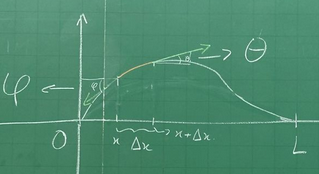
\includegraphics[height=0.5\textheight, width=0.5\textwidth, keepaspectratio]{./Images/vibrating_string_11.png}
	\end{center}
	\caption{ilustração de uma corda presa nas duas extremidades, com comprimento total L.}
	\label{vibestring11}
\end{figure}

Continuando com a ideia da física, é esperado que a força realizada para fazer a corda vibrar verticalmente resulte das componentes verticais da tração, que, seguindo o desenho, seriam descritas por
\[
	F = T\sin^{}{(\theta )} - T \sin^{}{(\varphi )}.
\]
Além disso, usando as estimativas para massa e aceleração acima, juntas à Segunda Lei de Newton, temos
\[
	Ma = T\sin^{}{(\theta )} - T \sin^{}{(\varphi )} \Rightarrow \rho \Delta x \frac{\partial^{2}u}{\partial t^{2}}(x, t) = T\sin^{}{(\theta )} - T \sin^{}{(\varphi )}.
\]
Podemos assumir que as vibrações sejam pequenas, resultando nos ângulos serem pequenos o suficiente para estimarmos que o seno e a tangente coincidem, tal que
\[
	\rho \Delta x \frac{\partial^{2}u}{\partial t^{2}}(x, t) \approx T \tan^{}{(\theta )} - T \sin^{}{(\theta )}
\]
e, como a tangente pode ser representada em termos da derivada, concluímos que
\[
	\rho \Delta x \frac{\partial^{2}u}{\partial t^{2}}(x, t) \approx T \frac{\partial^{}u}{\partial x^{}}(x+\Delta x, t) - T \frac{\partial^{}u}{\partial x^{}}(x, t).
\]
Portanto,
\[
	\rho \frac{\partial^{2}u}{\partial t^{2}}(x, t) = T \frac{\frac{\partial^{}u}{\partial x^{}}(x, t)-\frac{\partial^{}u}{\partial x^{}}(x, t)}{\Delta x},
\]
tal que, passando o limite conforme \(\Delta x\) torna-se minúscula,
\[
	\rho\frac{\partial^{2}u}{\partial t^{2}}(x, t) = T \frac{\partial^{2}u}{\partial x^{2}} \Longleftrightarrow \frac{\partial^{2}u}{\partial x^{2}}= \frac{T}{\rho }\frac{\partial^{2}u}{\partial x^{2}}.
\]

\begin{tcolorbox}[
		skin=enhanced,
		title=Lembrete!,
		after title={\hfill Aproximando Funções Trigonométricas},
		fonttitle=\bfseries,
		sharp corners=downhill,
		colframe=black,
		colbacktitle=yellow!75!white,
		colback=yellow!30,
		colbacklower=black,
		coltitle=black,
		%drop fuzzy shadow,
		drop large lifted shadow
	]
	O raciocínio acima pode parecer heresia, mas a lógica dele vem das séries de Taylor de seno e tangente:
	\begin{align*}
		 & \sin^{}{(\theta )} = \theta - \frac{\theta^{3}}{3} + \mathcal{O}(\theta^{5})  \\
		 & \tan^{}{(\theta )} = \theta + \frac{\theta^{3}}{3} + \mathcal{O}(\theta^{5}).
	\end{align*}
	Assim,
	\[
		\sin^{}{(\theta )} = \tan^{}{(\theta )} - \frac{2\theta^{3}}{3} + \mathcal{O}(\theta^{5})
	\]
	e, para \(\theta \) pequeno o suficiente, os termos ao cubo e à quinta desaparecem, deixando
	\[
		\sin^{}{(\theta )}\approx \tan^{}{(\theta )}.
	\]
	O termo denotado por um ``o'' maiúsculo chique é a chamada \textit{notação big-O}, para a qual há um lembrete logo a seguir
\end{tcolorbox}
\begin{tcolorbox}[
		skin=enhanced,
		title=Lembrete!,
		after title={\hfill Notação big-O e little-O},
		fonttitle=\bfseries,
		sharp corners=downhill,
		colframe=black,
		colbacktitle=yellow!75!white,
		colback=yellow!30,
		colbacklower=black,
		coltitle=black,
		%drop fuzzy shadow,
		drop large lifted shadow
	]
	A notação big-O, ou Ozão\footnote{Acho que ninguém chama assim, mas uma tradução livre seria quase isso}, determina o comportamento do limite de uma função conforme seus valores tendem a algum lugar. Formalmente falando, dizemos que \textbf{f(x) é da ordem (big-O) de g(x)} dado que existe um número real positivo M e um valor \(x_{0}\) dentro do domínio de f tais que
	\[
		|f(x)|\leq M|g(x)| \quad \forall x\geq x_{0}.
	\]
	Rearranjando isso, vemos que isto significa que, a partir de certo ponto no domínio da f, ela está a uma razão não maior que M da g:
	\[
		\frac{|f(x)|}{|g(x)|} \leq M \quad \forall x\geq x_{0},
	\]
	que permite definirmos que ``f é da ordem de g'' em termos do limite-supremo da razão, ou
	\[
		\limsup_{x\to \infty}\frac{|f(x)|}{|g(x)|} < \infty.
	\]
	Em ambos os casos, escrevemos \(f(x) = \mathcal{O}(g(x))\). Caso não estejamos interessados no limite ao infinito, podemos reformular isso conforme x tende a um valor a usando
	\[
		\limsup_{x\to a} \frac{|f(x)|}{|g(x)|} < \infty,
	\]
	para o qual escrevemos
	\[
		f(x) = \mathcal{O}(g(x)): x\rightarrow a.
	\]

	Existe também a notação little-O, ou Ozinho\footnote{Novamente uma tradução livre}, que é quase a big-O, mas restrita - a little-O está para a big-O assim como ``menor'' está para ``menor ou igual'', então seria
	\[
		\frac{|f(x)|}{|g(x)|} < M \quad \forall x\geq x_{0},
	\]
\end{tcolorbox}

\subsection{Unicidade da Equação da Onda}
Agora que vamos trabalhar com a unicidade da equação da onda, é bom mantermos muito bem definido o problema a ser analisado: consideraremos o seguinte problema de contorno:
\[
	\left\{\begin{array}{ll}
		{\color{blue}\frac{\partial^{2}u}{\partial t^{2}}(x, t) = \Delta u(x, t) + f(x, t),} & \quad t\in \mathbb{R},\; x\in \Omega           \\
		{\color{red}u(x, t) = h(x, t)},                                                      & \quad t\in \mathbb{R}, \; x\in \partial \Omega \\
		{\color{green}u(x, 0) = u_{0}(x)},                                                   & \quad x\in \Omega                              \\
		{\color{green}\frac{\partial^{}u}{\partial t^{}}(x, 0) = u_1(x)},                    & \quad x\in \Omega .
	\end{array}\right.
\]
Em azul, temos a {\color{blue} equação da onda em si}; em vermelho, a {\color{red}condição de contorno}; e, em verde, as {\color{green}condições iniciais}.
Sendo assim, podemos começar o estudo por meio da proposição a seguir

\begin{prop*}
	Existe no máximo uma solução da equação da onda, dada por uma função u de classe \(\mathcal{C}^{2}(\overline{\Omega }\times \mathbb{R})\), sendo \(\Omega \) um aberto regular limitado.
\end{prop*}
\begin{proof*}
	Sejam \(u, v\) duas funções de classes \(\mathcal{C}^{2}(\overline{\Omega }\times \mathbb{R})\) que solucionam a equação da onda. Defina
	\[
		w\coloneqq u - v,
	\]
	tal que
	\[
		\frac{\partial^{2}w}{\partial t^{2}} = \frac{\partial^{2}u}{\partial t^{2}} - \frac{\partial^{2}v}{\partial t^{2}} = \Delta u + f - \Delta v - f = \Delta u - \Delta v = \Delta w.
	\]
	Para t real e x na fronteira de \(\Omega \), vemos que w satisfaz a condição de fronteira
	\[
		w(x, t) = u(x, t) - v(x, t) = h(x, t) - h (x, t) = 0
	\]
	e, para y em \(\Omega \), as condições iniciais
	\begin{align*}
		 & w(y, 0) = u(y, 0) - v(y, 0) = u_{0}(y) - u_{0}(y) = 0                                                                                                 \\
		 & \frac{\partial^{}w}{\partial t^{}}(y, 0) = \frac{\partial^{}u}{\partial t^{}}(y, 0) = \frac{\partial^{}v}{\partial t^{}}(y, 0) = u_1(y) - u_1(y) = 0.
	\end{align*}
	\hypertarget{next_class_11}{\textit{Continua na próxima aula...}}
\end{proof*}
\end{document}
